\chapter{Results}
In order to visually demonstrate the encryption, visualisations of the ciphertext polynomial $c_0$ (refer to \autoref{sec:ckks}) were generated using a CRT decomposition of the RNS representation of $c_0$.
Each pixel corresponds to a coefficient $a \in \Z / q\Z$ scaled down by the modulus $q$ to obtain a brightness value between $0$ and $1$.

\begin{figure}[H]
  \centering
  \pgfplotsset{/pgfplots/group/.cd,vertical sep=1.6cm}
  \inputtikz{figures/generated/training-history}
  \caption{Development of the classification accuracy and the mean squared error during training.}
\end{figure}

\begin{figure}[H]
  \centering
  \inputtikz{figures/generated/confusion-matrix}
  \caption{Confusion Matrix of the trained network.}
\end{figure}

\begin{figure}[H]
  \centering
  % 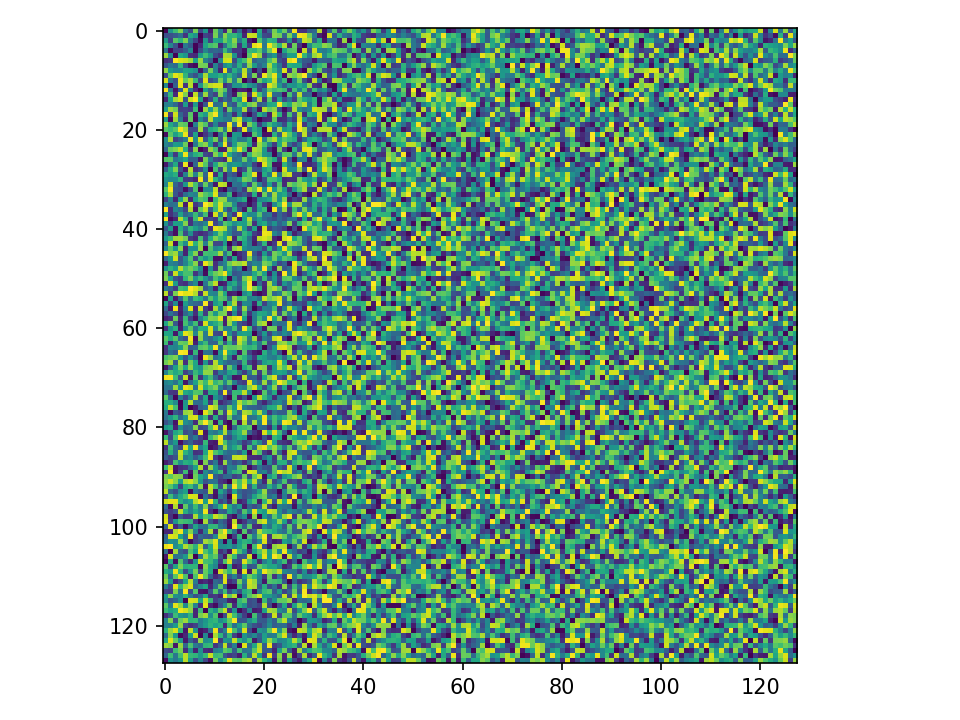
\includegraphics[width=\linewidth]{figures/ciphertext-visualisation.png}
  \inputtikz{figures/ciphertext-visualisation}
  \caption{Ciphertext Visualisation}
\end{figure}

\section{Methodology}
% TODO

\section{Accuracy, Precision, Recall}
% Detailliertere Analyse
% https://medium.com/analytics-vidhya/accuracy-precision-and-recall-in-machine-learning-classification-ae84004e86a1
% https://en.wikipedia.org/wiki/Precision_and_recall

\section{Performance Benchmarks}
This chapter includes runtime and communication overhead analysis.

Plain runtime: xxx

\begin{table}[H]
  \centering
  \caption{Performance Benchmarks / Communication Overhead}
  \begin{tabular}{lllll}
    \textbf{Scenario} & \textbf{Parameters} & \textbf{Runtime} / \si{\second} & \textbf{Message Size} / \si{\mega\byte} & \textbf{MRE} \\
    BSGS Matmul       & 60,40,...,40,60     &                                 &                                         &              \\
    BSGS Matmul       & 34,25,...,25,34     &                                 &                                         &              \\
    Hybrid Matmul     &                     &                                 &                                         &              \\
    Encrypt           &                     &                                 &                                         &              \\
    Encrypt Symmetric &                     &                                 &                                         &              \\
  \end{tabular}
\end{table}
